\FloatBarrier

\section{Introduction}
The CLAS12 Forward Calorimeters are used to stop high energy electrons and photons by sampling a portion of their electromagnetic showers.  The showers are created using interleaved layers of lead and plastic scintillator strips, where a fraction of the total shower energy sampled by the scintillators is converted to light and transported to photomultiplier tubes (PMT) for conversion to digital signals.  As a part of the calibration procedure, it is necessary to measure the attenuation of the light as it propagates down the length of each stack of scintillator strips.  This procedure also includes measurement of the gains of the PMTs.  This document describes the initial calibration measurements for the new CLAS12 designed calorimeter module, referred to as the Preshower Calorimeter (PCAL).

\section{Design}
The CLAS12 PCAL is triangular in shape and installed in front of the CLAS6 EC module.. The triangular form is isosceles (not equilateral), which was chosen
to better match the EC design and space limitations. A diagram of the front and side views of the PCAL with respect to the EC can be seen in 
Fig.~\ref{fig:geomfig1}. 

\begin{figure}[h]
    \centering
    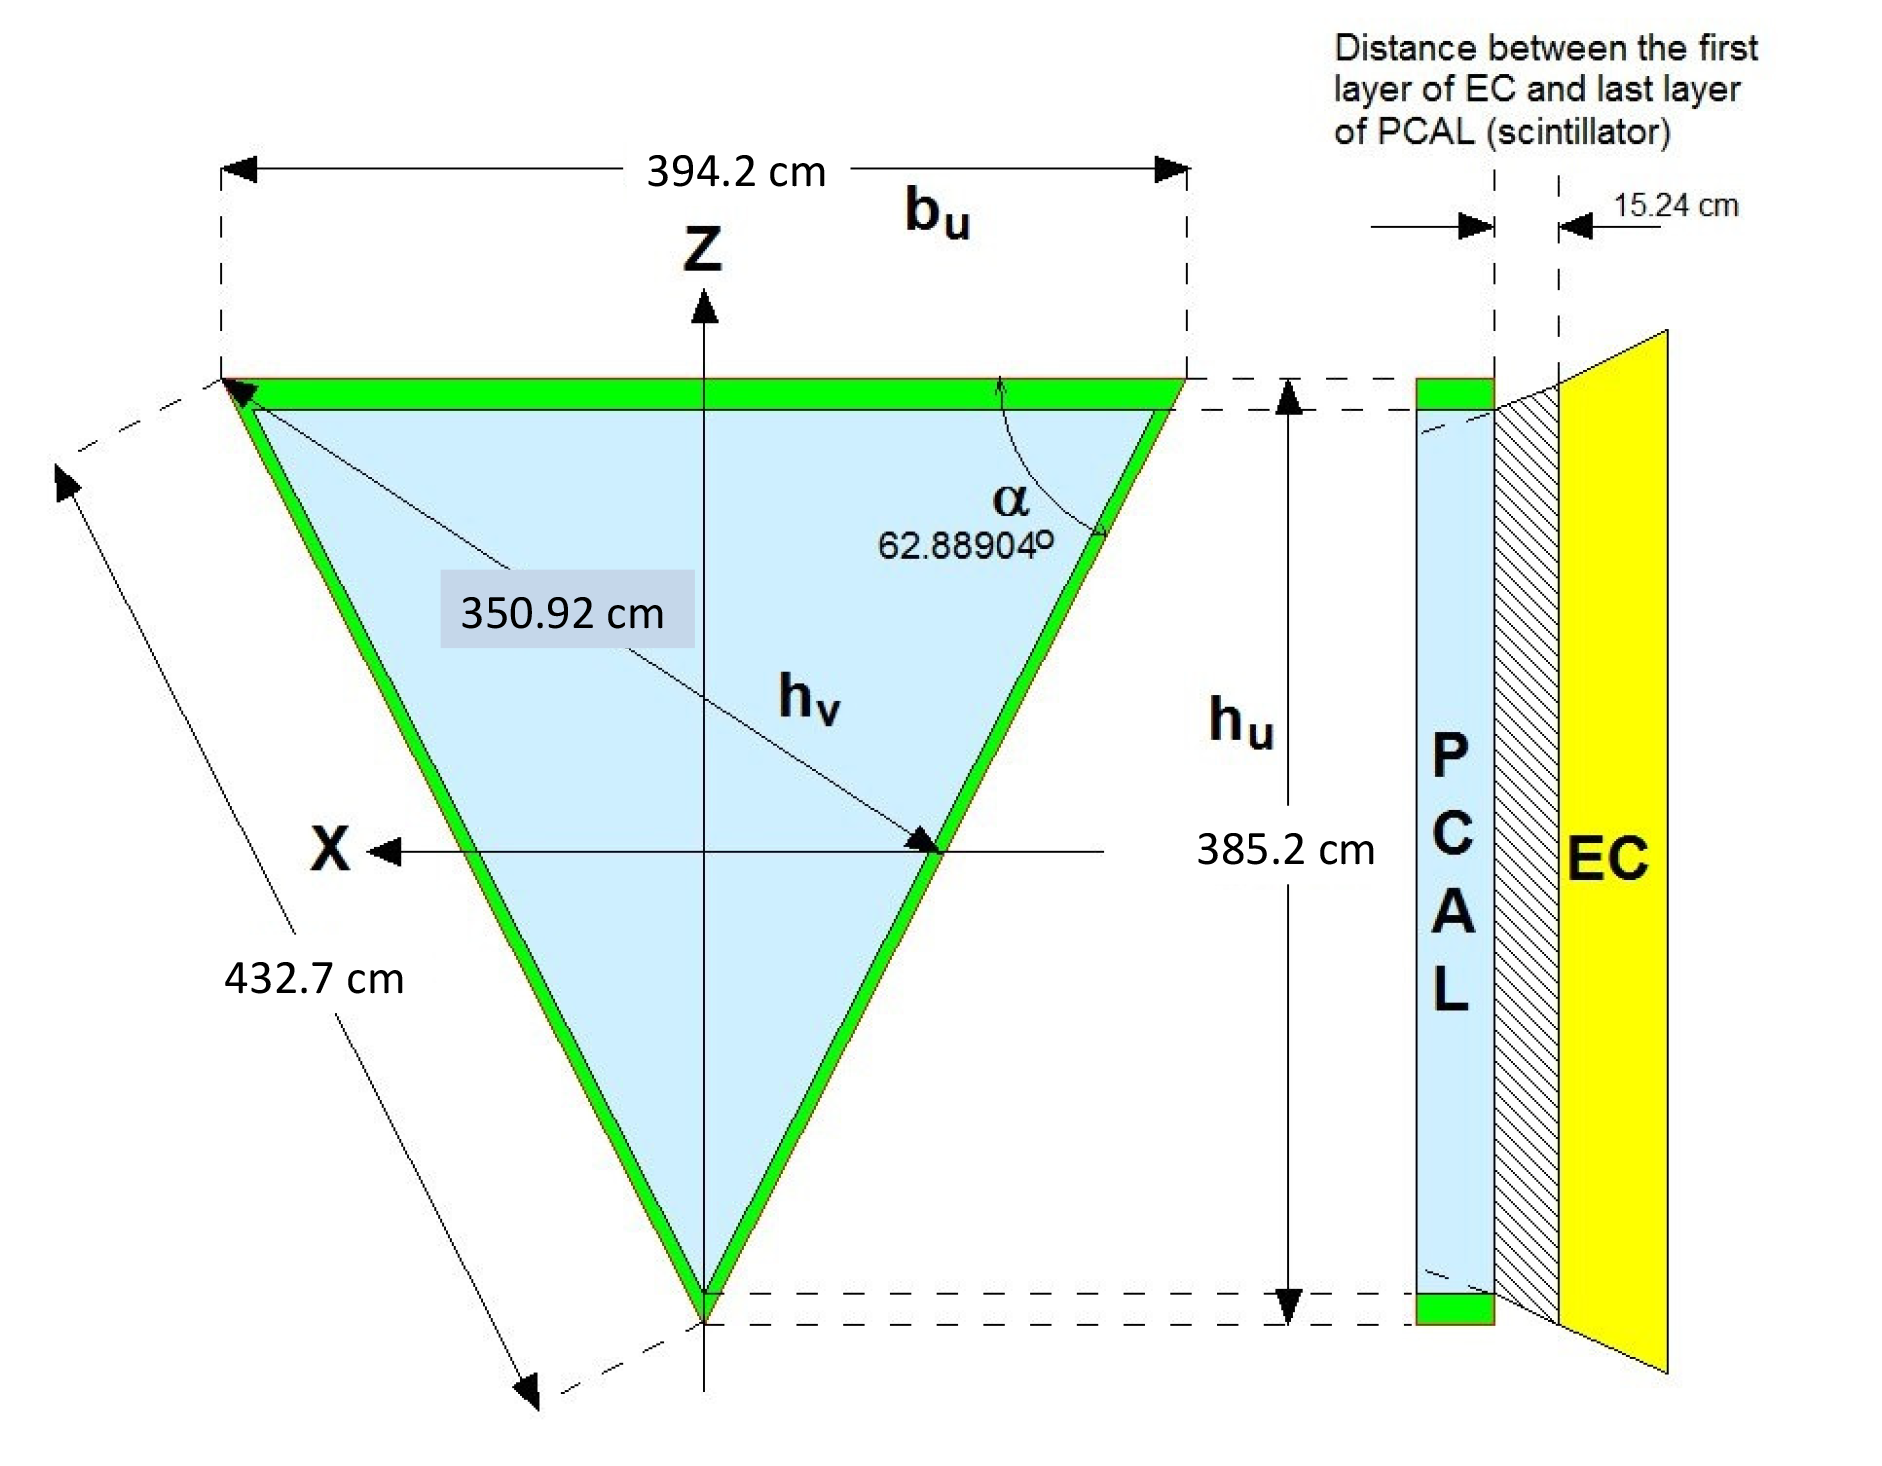
\includegraphics[width= 5in, keepaspectratio = true]{Pcal_geom_fig1}
    \caption{Front and side dimensions of the PCAL (from the PCAL geometry note~\cite{bib:geomnote}).}
    \label{fig:geomfig1}
\end{figure}

The PCAL box contains alternating layers of 1 cm thick scintillator strips and 0.22 cm thick lead sheets. Each scintillator layer has a readout orientation rotated with respect to the previous layer. These orientations are described as the U, V, and W layers. Each layer is parallel with one side of the PCAL box. The sequence (U,lead,V,lead,W,lead) is repeated five times within a single PCAL module. This results in a 15 layer lead/scintilator 'sandwich' as shown in Fig.~\ref{fig:geomfig4}.

\begin{figure}[h]
    \centering
    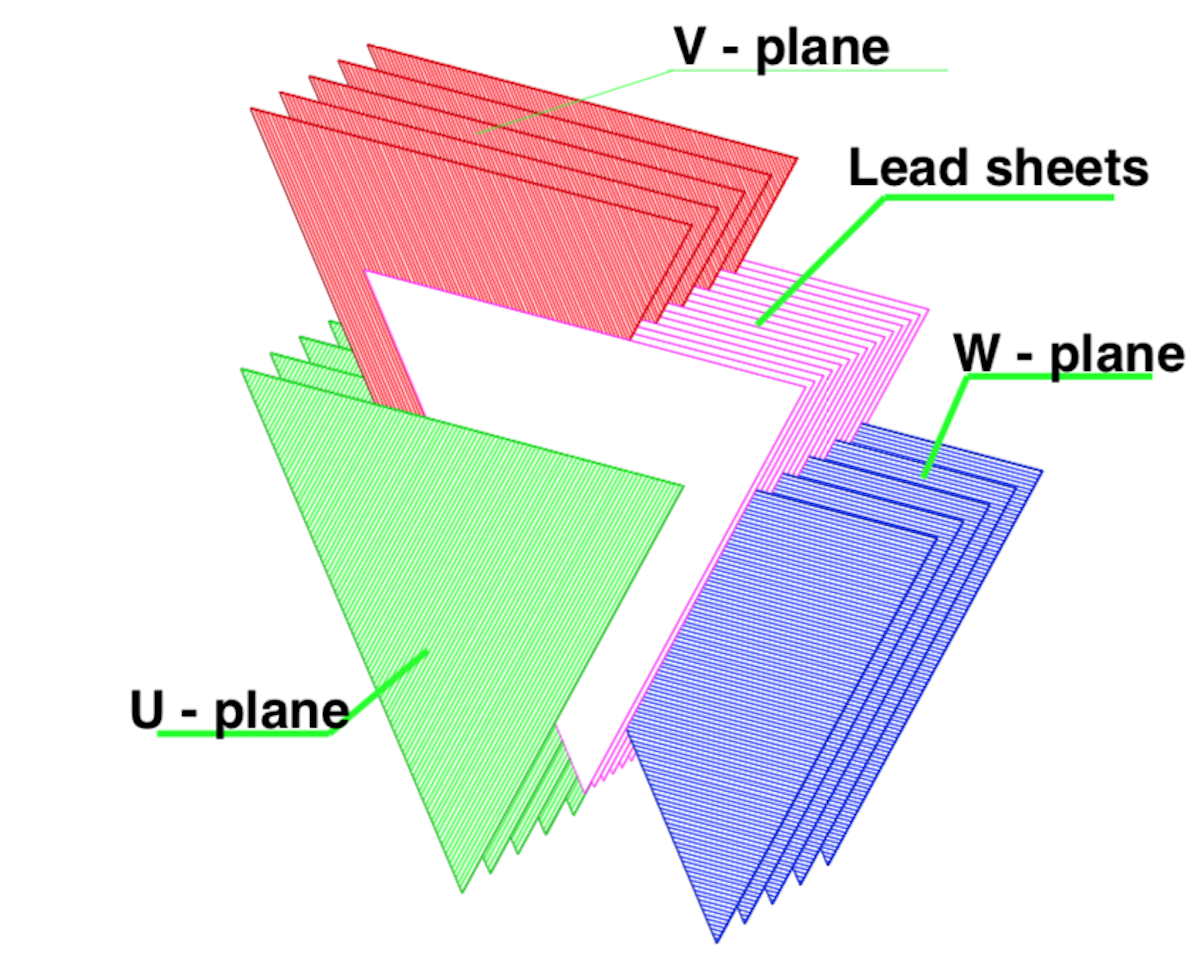
\includegraphics[width= 3in, keepaspectratio = true]{pcal_layers}
    \caption{Schematic showing interleaving of U,V,W scintillator layers with lead.}
    \label{fig:geomfig4}
\end{figure}

\FloatBarrier
\begin{figure}[h]
    \centering
    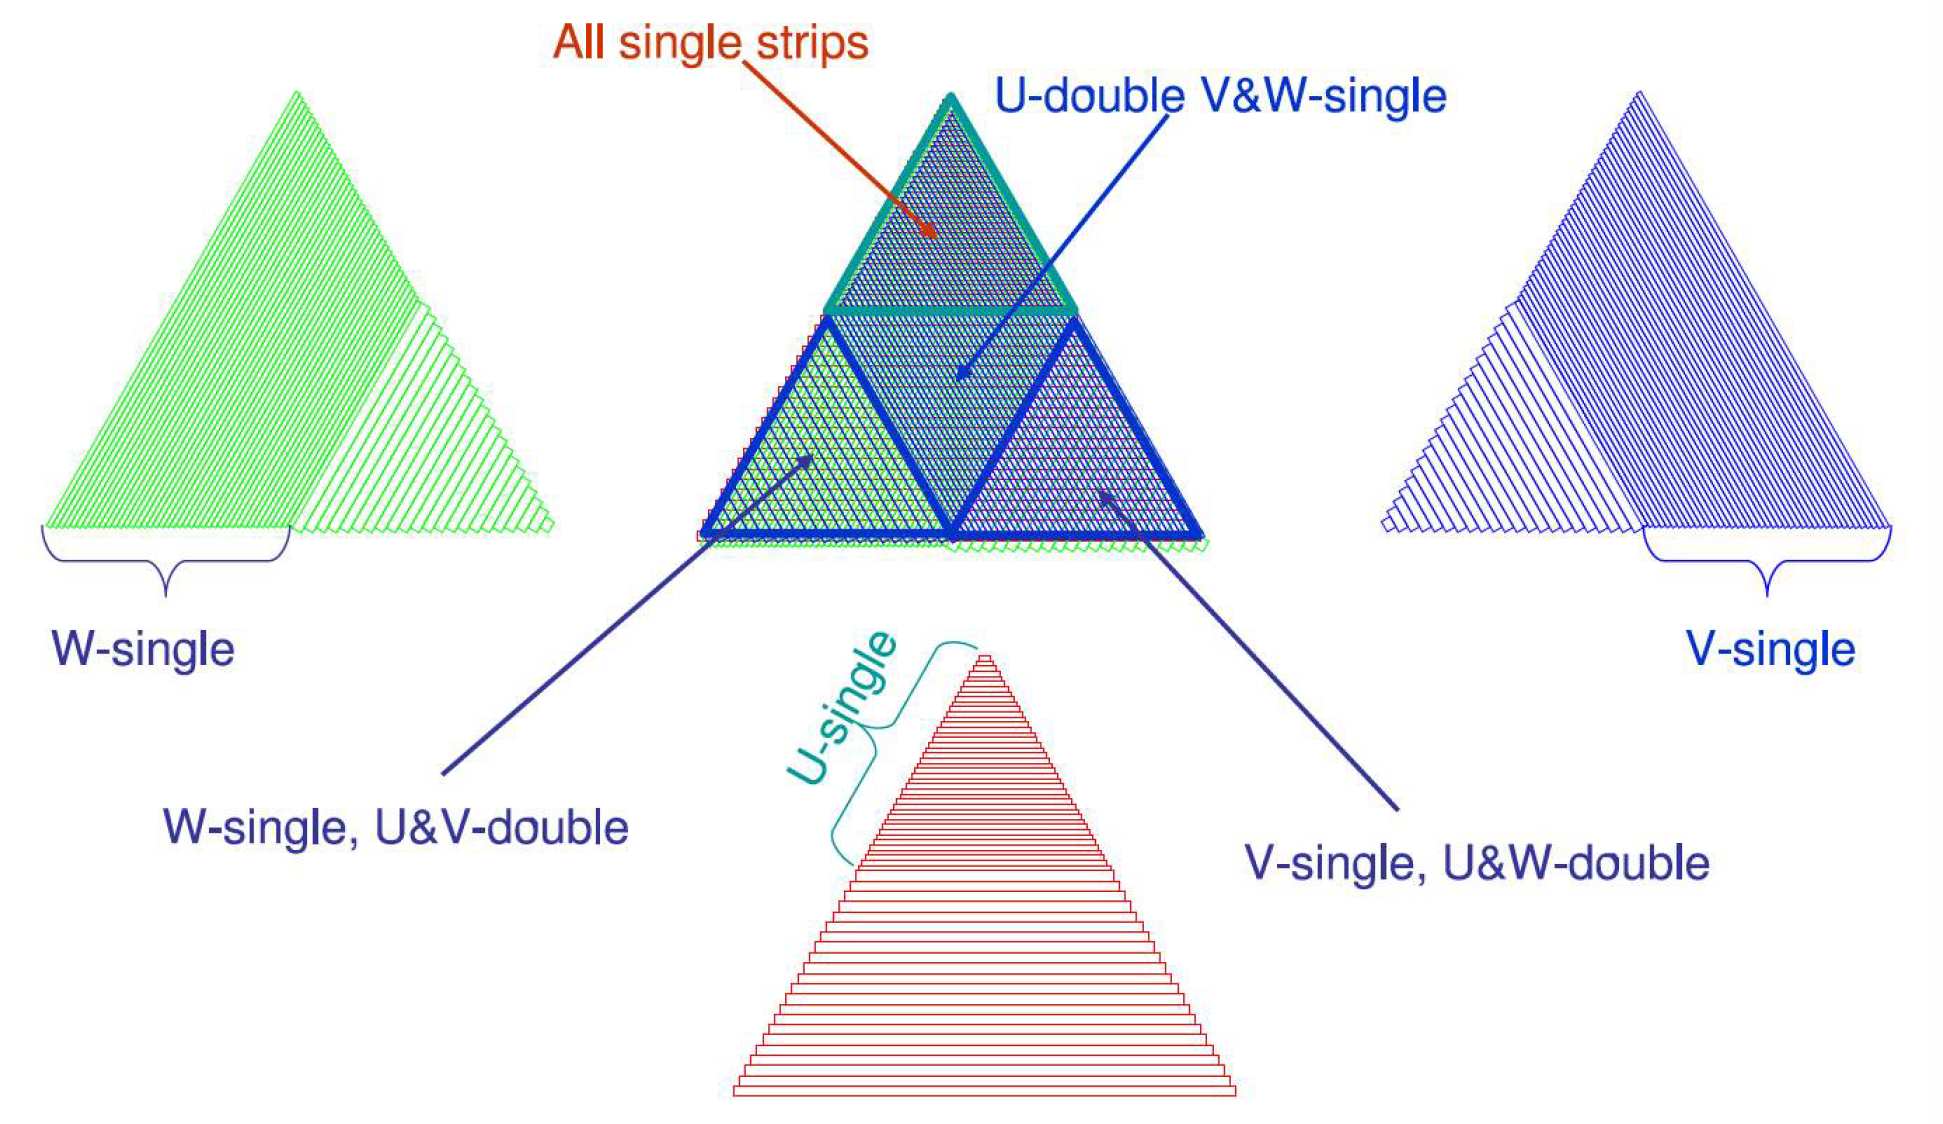
\includegraphics[width= 5in, keepaspectratio = true]{Pcal_geom_fig5}
    \caption{Orientation and readout size of scintillator strips~\cite{bib:geomnote}.}
    \label{fig:geomfig5}
\end{figure}
\FloatBarrier

\FloatBarrier
There are 84 U strips, 77 V strips, and 77 W strips in each corresponding layer. The readout from the last 32 U strips are grouped in pairs into a single PMT per pair. The first 30 V and W strips are also grouped in pairs within their respective layer. As a consequence 
there is better spatial resolution for low strip numbers in the U layer and for high strip numbers in the V and W layers. Each of the five repeating layer strip readouts is coupled to the same PMT, which sums the five different signals. This readout pattern of scintillators is illustrated in Fig.~\ref{fig:geomfig5}.

Due to this grouping of scintillator strips, our numbering scheme uses the PMT receiving the readout fibers. Thus U PMTs 1-52 readout individual 'single' strips, while U PMTs 53-68 readout 'double' strips. Lower numbered PMTs readout shorter strips while higher numbered PMTs readout the longer strips.  For example, V1 is the shortest and V62 is the longest strip in the V view. This strip convention is used throughout this document and is taken from the PCAL geometry note~\cite{bib:geomnote}. Using this convention, the layout of the PMT readout can easily be understood from Fig.~\ref{fig:PMTreadout} which shows PMT readout of a strip in each view.
\begin{figure}[h]
    \centering
    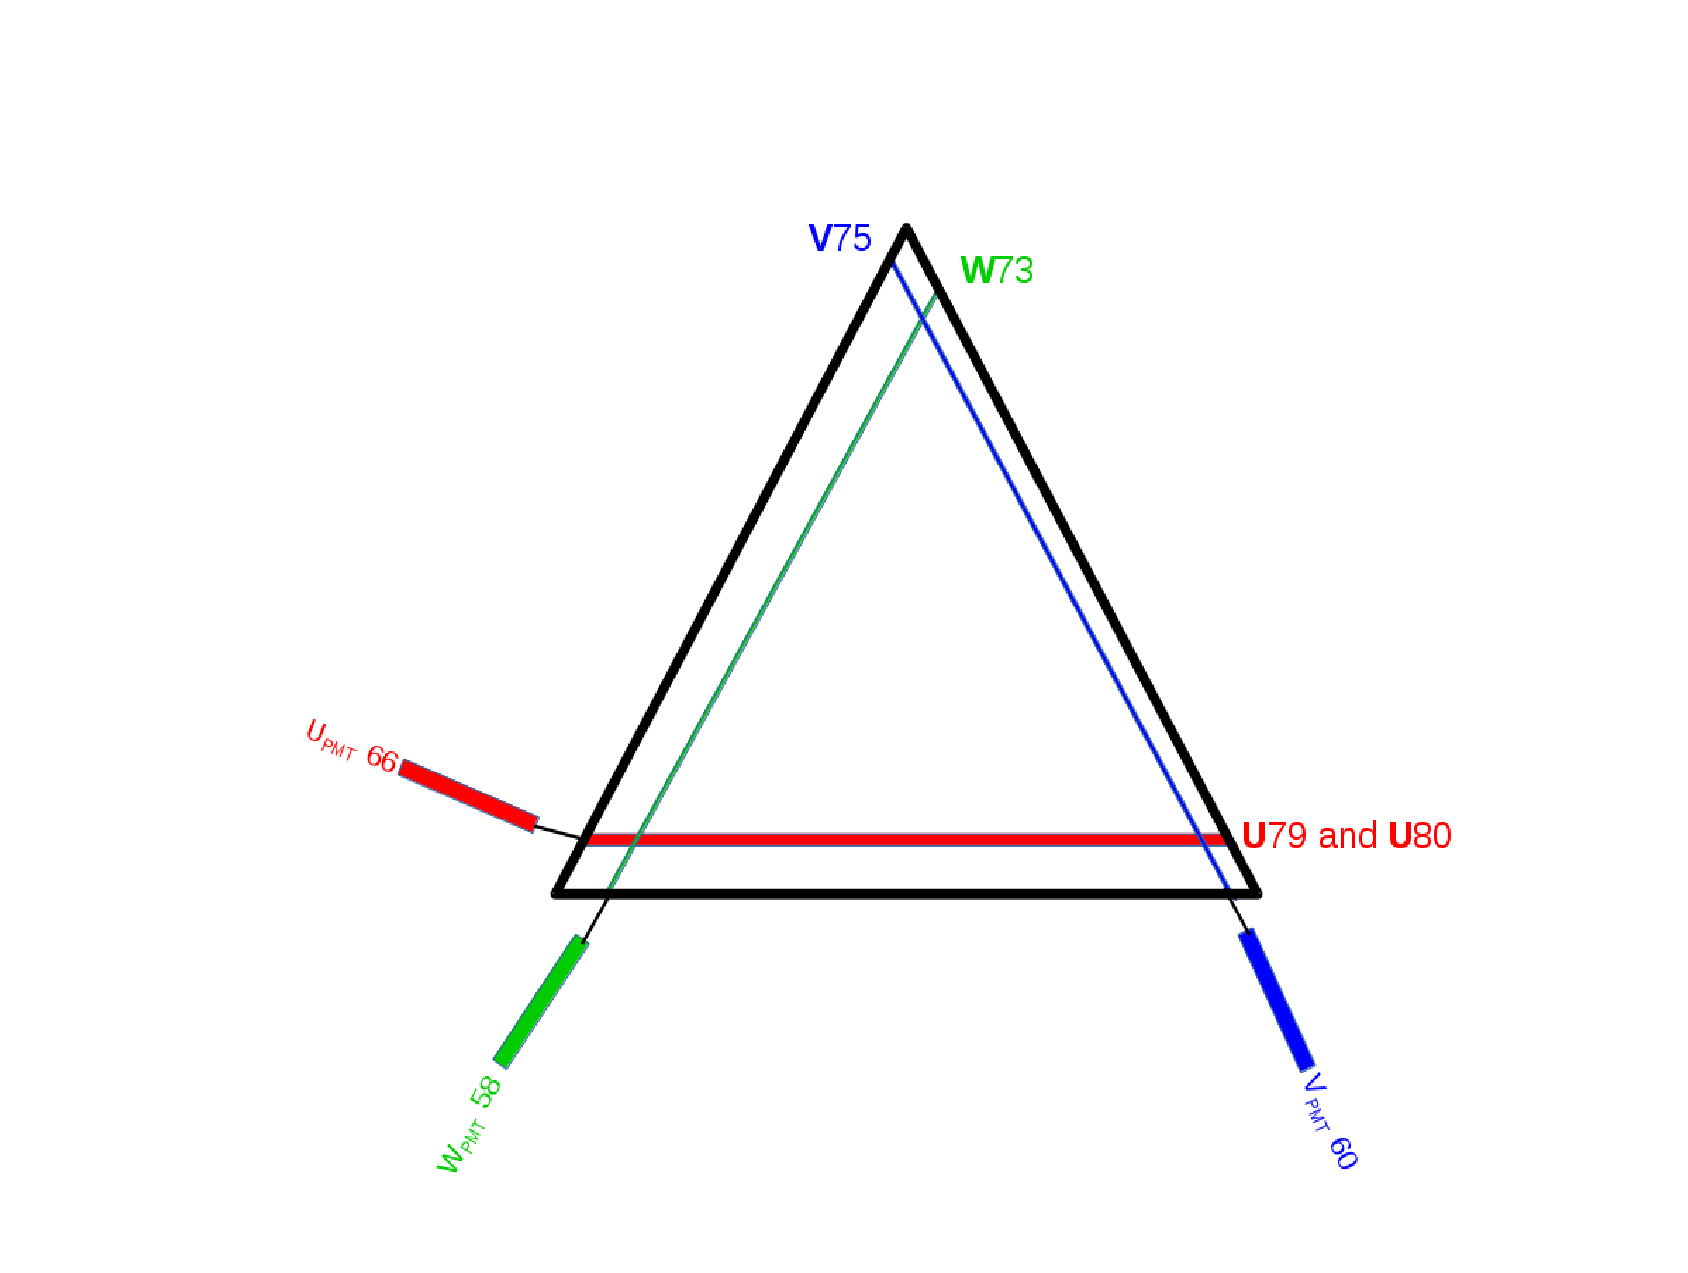
\includegraphics[width= 4.5in, keepaspectratio = true]{PMTreadout}
    \caption{Cartoon showing the layout of the PMT readout for different views.}
    \label{fig:PMTreadout}
\end{figure}
\FloatBarrier


\section{Cosmic Ray Tests}
Assembly of six PCAL modules occurred in 2012-2013 in Room 26 of the EEL building.  After assembly each module was moved to the cosmic-ray test (CRT) area where PMTs were installed and connected to a DAQ system for initial testing.  A loose trigger was setup using the OR of all W strip PMTs, with the trigger threshold adjusted to reject low energy pulses.  This choice of W increased the probability that the cosmic muons penetrated the U,V layers and the threshold setting helped reject non-perpendicular tracks.
\begin{figure}[h]
    \centering
    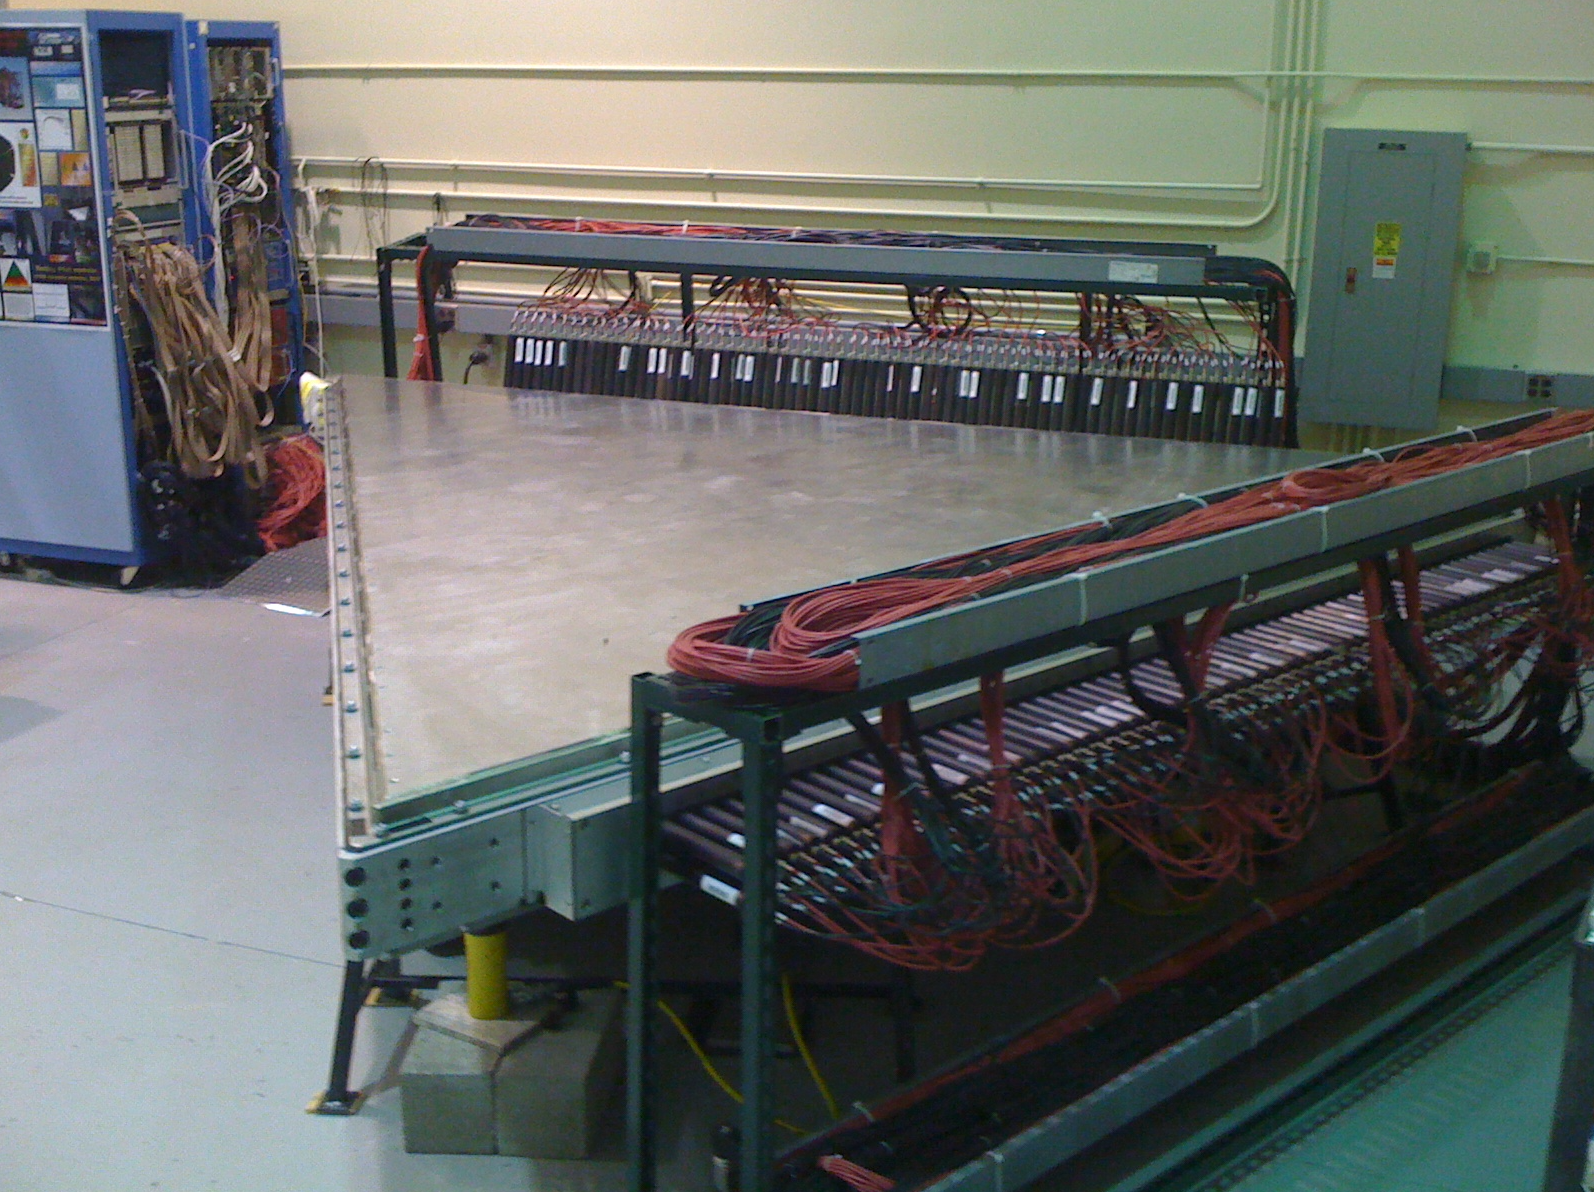
\includegraphics[width= 3.5in, keepaspectratio = true]{pcal3}
    \caption{PCAL MODULE 3 - Tested July 2012. Installed as Sector 2 in HallB.}
    \label{fig:pcal3}
\end{figure}

During these tests procedures were developed to gain match the PMTs by using the hodoscope function of the calorimeter to isolate perpendicular cosmic muon hits at a fixed distance from the end of the scintillator strips. This resulted in a constant minimum ionizing energy of 10 MeV deposited in the five scintillators making up each U,V,W stack.  The PMT HV was adjusted until each PMT produced a MIP peak in channel 200 of the ADC distributions within an error of $\pm$5\%.  Attention was then turned to performing long runs to accumulate enough data to perform measurements of light attenuation constants.  

\clearpage
